\documentclass[11pt]{article}
\title{\textbf{Triple unit}}
\author{https://github.com/heptagons/meccano/units/triple}
\date{}

\usepackage{../../meccano}
\usepackage{tikz}
\usetikzlibrary{calc}

\begin{document}

\maketitle
\begin{abstract}
Triple unit is a group of five meccano\meccanoref strips $a,b,c,d,e$ intended to build regular polygons three consecutive perimeter sides.
This unit has three angles equal to the polygon internal angle $\theta$. 
Triple unis has been using to build the pentagon type 2 mentioned in pentagons paper\footnote{
\href{https://github.com/heptagons/meccano/blob/main/penta/pentagons.pdf}{Meccano pentagons}}.
\end{abstract}

\begin{figure}[h]
\centering
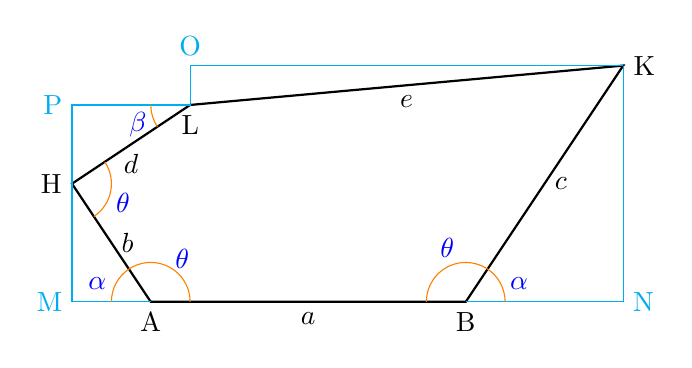
\begin{tikzpicture}
\begin{scope}[scale=0.5]
\draw[black,thick] (0,0)
-- node[below] {$a$} ++(8,0) node[below]{B}
-- node[below,right] {$c$} ++(4,6) node[right]{K}
-- node[below] {$e$} ++(-11,-1) node[right,below]{L}
-- node[below] {$d$} ++(-3,-2) node[left]{H}
-- node[right] {$b$} cycle node[below]{A};
\draw[cyan] (0,0)
-- ++(-2,0) node[below,left] {M}
-- ++(0,3)
-- ++(0,2) node[above,left] {P}
-- ++(3,0)
-- ++(0,1) node[above] {O}
-- ++(11,0);
\draw[cyan] (8,0)
-- ++(4,0) node[below,right] {N}
-- ++(0,6);

\draw[orange] (0,0)+(-1,0)
 arc(180:180-atan(3/2):1) node[midway,above,left,blue] {$\alpha$}
 arc(180-atan(3/2):0:1) node[above,blue,pos=0.7] {$\theta$};
\draw[orange] (8,0)+(-1,0)
 arc(180:atan(3/2):1) node[above,blue,pos=0.5] {$\theta$}
 arc(atan(3/2):0:1) node[midway,above,right,blue] {$\alpha$};
\draw[orange] (-2,3)+(0.832,0.554) %sin(atan(3/2),cos(atan(3/2))
 arc(atan(2/3):-atan(3/2):1) node[right,blue,pos=0.7] {$\theta$};
\draw[orange] (1,5)+(-0.832,-0.554)
 arc(180+atan(2/3):180:1) node[left,blue,pos=0.1] {$\beta$};
\end{scope}
\end{tikzpicture}
\caption{Triple unit has five strips $a,b,c,d,e$}
\label{fig:triple}
\end{figure}

\section{Algebra}

From nodes $A$ and $B$ of fig \ref{fig:triple} we get $\alpha$ from $\theta$ ($\pi = 180^\circ$):
\begin{align}
\theta &= \pi - \alpha \nonumber\\
\alpha &= \pi - \theta
\end{align}
And from node $H$ we get $\beta$ from $\theta$:
\begin{align}
\theta &= \alpha + \beta \nonumber\\
\beta &= \theta - \alpha = \theta - (\pi - \theta) = 2\theta - \pi
\end{align}

We calculate horizontal segment $\overline{OK}$:
\begin{align}
\overline{OK} &= \overline{MA} + a + \overline{BN} - \overline{PL} \nonumber\\
 &= b\cos{\alpha} + a + c\cos{\alpha} - d\cos{\beta} \nonumber\\
 &= a + (b+c)\cos{\alpha} - d\cos{\beta} \nonumber\\
 &= a + (b+c)\cos{(\pi-\theta)} - d\cos{(2\theta - \pi)} \nonumber\\
 &= a - (b+c)\cos{\theta} + d\cos{(2\theta)}
\end{align} 

And vertical segment $\overline{OL}$:
\begin{align}
\overline{OL} &= \overline{KN} - \overline{PH} - \overline{HM} \nonumber\\
 &= c\sin{\alpha} - d\sin{\beta} - b\sin{\alpha} \nonumber\\
 &= (c-b)\sin{\alpha} - d\sin{\beta} \nonumber\\
 &= (c-b)\sin{(\pi-\theta)} - d\sin{(2\theta-\pi)} \nonumber\\
 &= (c-b)\sin{\theta} + d\sin{(2\theta)}
\end{align}

So we can express $e$ in function of $a,b,c,d$ and angle $\theta$:
\begin{align}
e^2 &= (\overline{OK})^2 + (\overline{OL})^2 \nonumber\\
 &= (a -(b+c)\cos\theta +d\cos(2\theta))^2 +((c-b)\sin\theta +d\sin(2\theta))^2 \nonumber\\
 &= a^2 +(b^2+2bc+c^2)\cos^2\theta + d^2\cos^2(2\theta) + (c^2-2cb+b^2)sin^2\theta +d^2\sin^2(2\theta) \nonumber\\
 &\qquad -2a(b+c)\cos\theta +2ad\cos(2\theta) -2(b+c)d\cos\theta\cos(2\theta) \nonumber\\
 &\qquad +2(c-b)d\sin\theta\sin(2\theta) \nonumber\\
%
 &= a^2 +b^2 +c^2 +d^2 +2bc\cos^2\theta -2bc\sin^2\theta \nonumber\\
 &\qquad -2a(b+c)\cos\theta +2ad\cos(2\theta) \nonumber\\
 &\qquad -2d((b+c)\cos\theta\cos(2\theta) + (b-c)\sin\theta\sin(2\theta)) \\
%
 &= a^2 +b^2 +c^2 +d^2 +2bc(\cos^2\theta -\sin^2\theta) 
  -2a(b+c)\cos\theta +2ad\cos(2\theta) \nonumber\\
 &\qquad -2d(b(\cos\theta\cos(2\theta)+\sin\theta\sin(2\theta)) 
  + c(\cos\theta\cos(2\theta)-\sin\theta\sin(2\theta))) \nonumber\\
%  
 &= a^2 +b^2 +c^2 +d^2 +2bc\cos(2\theta) 
  -2a(b+c)\cos\theta +2ad\cos(2\theta) \nonumber\\
 &\qquad -2d(b\cos(\theta-2\theta) + c\cos(\theta+2\theta)) \nonumber\\
% 
 &= a^2 +b^2 +c^2 +d^2 +2(bc+ad)\cos(2\theta) -2a(b+c)\cos\theta -2d(b\cos\theta + c\cos(3\theta)) \nonumber\\
% 
 &= a^2 +b^2 +c^2 +d^2 +2(bc+ad)\cos(2\theta) -2(ab+ac)\cos\theta -2(bd\cos\theta + cd\cos(3\theta)) \nonumber\\
%
 &= \boxed{ a^2 +b^2 +c^2 +d^2 -2(ab+ac+bd)\cos\theta +2(bc+ad)\cos(2\theta) -2cd\cos(3\theta) }
\end{align}

\section{Regular polygons}

\begin{table}[h]
\centering
\begin{tabular}{|c c c c c|}\hline
Polygon & $\theta$ & $\cos\theta$ & $\cos(2\theta)$ & $\cos(3\theta)$ \rule[-2ex]{0pt}{6ex}\\ \hline\hline 
Pentagon & $\dfrac{3\pi}{5}$ & $\dfrac{1-\sqrt{5}}{4}$ & $\dfrac{-1-\sqrt{5}}{4}$ & $\dfrac{1+\sqrt{5}}{4}$\rule[-2ex]{0pt}{6ex}\\ \hline
Hexagon & $\dfrac{2\pi}{3}$ & $-\dfrac{1}{2}$ & $-\dfrac{1}{2}$ & $1$ \rule[-2ex]{0pt}{6ex}\\ \hline
Heptagon & $\dfrac{5\pi}{7}$ &  &  & \rule[-2ex]{0pt}{6ex}\\ \hline
Octagon & $\dfrac{3\pi}{4}$ &  &  & \rule[-2ex]{0pt}{6ex}\\ \hline
Decagon & $\dfrac{4\pi}{5}$ &  &  & \rule[-2ex]{0pt}{6ex}\\ \hline
Dodecagon & $\dfrac{5\pi}{6}$ &  &  & \rule[-2ex]{0pt}{6ex}\\ \hline

\end{tabular}
\caption{Regular polygons internal angles and cosines.}
\label{tbl:polygons}
\end{table}

\subsection{Equilateral pentagon}

We replace the cosines for pentagon in table \ref{tbl:polygons} in $e^2$ equation:
\begin{align}
e^2 &= a^2 +b^2 +c^2 +d^2 -2(ab+ac+bd)\cos\theta +2(bc+ad)\cos(2\theta) -2cd\cos(3\theta) \nonumber\\
 &= a^2 +b^2 +c^2 +d^2
  -2(ab+ac+bd)\left(\dfrac{1-\sqrt{5}}{4}\right)
  +2(bc+ad)\left(\dfrac{-1-\sqrt{5}}{4}\right)
  -2cd\left(\dfrac{1+\sqrt{5}}{4}\right) \nonumber\\
 &= a^2 +b^2 +c^2 +d^2 -\frac{ab+ac+bd+bc+ad+cd}{2} +\frac{ab+ac+bd-bc-ad-cd}{2}\sqrt{5}
\end{align}
$e$ cannot to be and integer if the factor of $\sqrt{5}$ is not zero so we force this factor to be zero:
\begin{align}
 ab+ac+bd-bc-ad-cd &= 0\nonumber\\
 ab+ac+bd &= bc+ad+cd
\end{align}
We replace $ab+ac+bd$ by $bc+ad+cd$ in the $e^2$ equation to get:
\begin{align}
e^2 &= a^2 +b^2 +c^2 +d^2 -\frac{(bc+ad+cd)+bc+ad+cd}{2} +\frac{0}{2}\sqrt{5} \nonumber\\
 &= a^2 +b^2 +c^2 +d^2 -bc -ad -cd \nonumber\\
e &= \sqrt{a^2 +b^2 +c^2 +d^2 -bc -ad -cd}
\end{align}
The last formula matches the formula used in the paper Meccano pentagons which finds several pentagons of type 2. 
Only when we get $e$ integer we have a solution.

\subsection{Equilateral hexagon}

We replace the cosines for hexagon in table \ref{tbl:polygons} in $e^2$ equation:
\begin{align}
e^2 &= a^2 +b^2 +c^2 +d^2 -2(ab+ac+bd)\cos\theta +2(bc+ad)\cos(2\theta) -2cd\cos(3\theta) \nonumber\\
 &= a^2 +b^2 +c^2 +d^2 -2(ab+ac+bd)\left(-\frac{1}{2}\right) +2(bc+ad)\left(-\frac{1}{2}\right) -2cd(1) \nonumber\\
 &= a^2 +b^2 +c^2 +d^2 +ab+ac+bd -bc-ad-2cd \nonumber\\
 &= (a+b)^2 +(c-d)^2 -ab+ac+bd-bc-ad\nonumber\\
 &= (a+b)^2 +(c-d)^2 +(c-d)(a-b) -ab \nonumber\\
 &= (a+b)^2 +(c-d)(a-b+c-d) -ab \nonumber\\
e &= \sqrt{(a+b)^2 +(c-d)(a-b+c-d) -ab}
\end{align} 





\end{document}